\documentclass[10pt,a4paper]{article}
\usepackage[utf8]{inputenc}
\usepackage[T1]{fontenc}
\usepackage[romanian]{babel}
\usepackage[margin=1.7cm]{geometry}
\usepackage{amsmath,amssymb}
\usepackage{enumitem}
\usepackage{titlesec}
\usepackage{parskip}
\usepackage{tikz}
\usepackage{circuitikz}
\usepackage{pgfplots}
\pgfplotsset{compat=1.18}
\usetikzlibrary{arrows.meta}
\usepackage[most]{tcolorbox}
\usepackage[colorlinks=true,linkcolor=red!55!black,urlcolor=red!55!black]{hyperref}
\newtcolorbox{keyeq}{colback=red!5,colframe=red!70!black,boxrule=0.7pt,arc=2pt,boxsep=2pt,left=5pt,right=5pt,top=3pt,bottom=3pt,boxsep=1pt,breakable}
\newtcolorbox{methodbox}{colback=blue!4,colframe=blue!55!black,boxrule=0.7pt,arc=2pt,boxsep=2pt,left=5pt,right=5pt,top=3pt,bottom=3pt,boxsep=1pt,breakable}
\newcommand{\tip}[1]{\textcolor{blue!55!black}{#1}}
\newcommand{\srcnote}[1]{{\footnotesize\color{gray!55!black}\textit{Sursă: #1}}\par}
\setlist{nosep, topsep=2pt, itemsep=2pt, leftmargin=1.4em}
\titlespacing*{\section}{0pt}{8pt}{4pt}
\titlespacing*{\subsection}{0pt}{6pt}{2pt}
\renewcommand{\baselinestretch}{0.97}
\pagestyle{plain}

\title{\vspace{-2cm}Rezumat examen SAE (Sisteme Discrete)}
\author{\large Compilat de Stefan Jipa}
\date{}

\begin{document}
\maketitle
\vspace{-1.2cm}

\section*{1. Sisteme discrete — noțiuni introductive}\phantomsection\label{sec:1}
\srcnote{curs 1 (secțiunea introductivă, fig. 4.1a/4.1b).}
\textbf{Sistem de reglare numeric} vs. \textbf{continuu}: la sistemul numeric procesarea legii de reglare se face cu ecuații algebrice recursive, în cadrul unui procesor numeric, pe eșantioane prelevate la momente discrete (nu pe semnal continuu).

\textbf{Elementele specifice unui sistem numeric} sunt convertoarele:
\begin{itemize}
\item \textbf{CA/N} (analog/numeric) — transformă semnalul analogic în secvență numerică (discretizată în timp \emph{și} amplitudine, reprezentată binar); include implicit eșantionare + cuantizare;
\item \textbf{CN/A} (numeric/analogic) — reconstituie semnalul continuu din cel numeric; procesul include și o filtrare trece-jos (FTJ) a semnalului discretizat.
\end{itemize}

\textbf{Schema bloc a unui sistem de reglare numeric (buclă cu eșantionarea erorii):}
\begin{center}
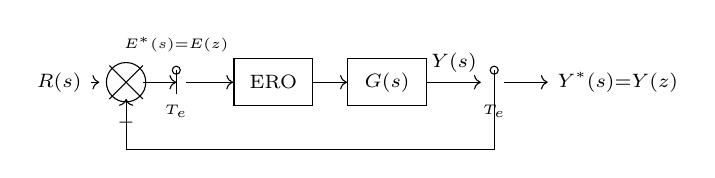
\begin{tikzpicture}[scale=0.85, every node/.style={font=\scriptsize}]
\node (r) at (0,0) {$R(s)$};
\draw[->] (r) -- (0.6,0);
\node[draw,circle,minimum size=0.5cm] (sum) at (1.0,0) {};
\draw (0.75,0.25)--(1.25,-0.25); \draw (0.75,-0.25)--(1.25,0.25);
\node[below] at (1,-0.35) {$-$};
\draw[->] (1.25,0) -- (1.75,0);
\draw (1.75,0.18) circle (0.06); \draw (1.75,-0.18)--(1.75,0.18);
\node[below] at (1.75,-0.2) {\tiny$T_e$};
\node[above] at (1.75,0.3) {\tiny$E^*(s){=}E(z)$};
\draw[->] (1.9,0) -- (2.6,0);
\node[draw,minimum width=1cm,minimum height=0.6cm] (ero) at (3.2,0) {ERO};
\draw[->] (3.8,0) -- (4.3,0);
\node[draw,minimum width=1cm,minimum height=0.6cm] (g) at (4.9,0) {$G(s)$};
\draw[->] (5.5,0) -- (6.3,0) node[above,pos=0.5]{$Y(s)$};
\draw (6.5,0.18) circle (0.06); \draw (6.5,-0.18)--(6.5,0.18);
\node[below] at (6.5,-0.2) {\tiny$T_e$};
\draw[->] (6.65,0) -- (7.3,0) node[right]{$Y^*(s){=}Y(z)$};
\draw[->] (6.5,0) |- (6.5,-1) -| (1,-1) -- (1,-0.25);
\end{tikzpicture}
\end{center}

\section*{2. Eșantionarea ideală și aliasing}\phantomsection\label{sec:2}
\srcnote{curs 2, secțiunea 4.2.1 (numerotare locală în fișierul sursă: „2.1") — eșantionare ideală, spectru, aliasing, teorema Shannon.}
\textbf{Eșantionorul ideal (EI)} — comutator sincron cu perioadă $T_e$, durată de închidere infinitezimală. Semnalul eșantionat ideal:
\begin{keyeq}\color{red!65!black}
$$f^*(t)=f(t)\,\delta_{T_e}(t)=\sum_{k=-\infty}^{\infty}f(kT_e)\delta(t-kT_e),\qquad \delta_{T_e}(t)=\sum_{k=-\infty}^{\infty}\delta(t-kT_e)$$
\end{keyeq}
Transformata Laplace: $F^*(s)=\sum_{k=0}^{\infty}f(kT_e)e^{-skT_e}=\dfrac{1}{T_e}\sum_{k=-\infty}^{\infty}F(s-jk\omega_e)$.

\textbf{Spectrul semnalului eșantionat:}
\begin{keyeq}\color{red!65!black}
$$F^*(j\omega)=\dfrac{1}{T_e}\sum_{k=-\infty}^{\infty}F\big(j(\omega-k\omega_e)\big),\qquad \omega_e=\dfrac{2\pi}{T_e}$$
\end{keyeq}
— o infinitate de replici ale spectrului continuu, ponderate cu $1/T_e$, centrate pe multiplii lui $\omega_e$.

\textbf{Aliasing:} fie $\omega_m$ pulsația maximă din spectrul semnalului continuu (bandă limitată).
\begin{itemize}
\item $\omega_e/2>\omega_m$ — lobii nu se suprapun, semnal recuperabil exact cu un FTJ ideal;
\item $\omega_e/2<\omega_m$ — lobii se suprapun (\textbf{aliasing}), informație pierdută ireversibil; erorile devin importante mai ales dacă semnalul are zgomot cu amplitudine mare.
\end{itemize}
\textbf{Pulsația Nyquist:} $\omega_N=\omega_e/2$. \textbf{Soluție anti-aliasing:} filtrare trece-jos a semnalului continuu \emph{înainte} de CA/N, care elimină complet componentele cu $\omega>\omega_e/2$.

\textbf{Teorema eșantionării (Shannon):}
\begin{keyeq}\color{red!65!black}
$$\omega_e\ge 2\omega_m \quad\text{(teoretic)}\qquad\qquad \omega_e/2\ge 5\omega_m\ \text{ adică } \omega_e\ge 10\,\omega_m\quad\text{(practic)}$$
\end{keyeq}

\section*{3. Cuantizarea în amplitudine}\phantomsection\label{sec:3}
\srcnote{curs 2, secțiunea 4.2.2.}
Fiecare eșantion $f(kT_e)$ e aproximat cu un multiplu întreg al pasului de cuantizare $q$:
\begin{itemize}
\item \textbf{prin rotunjire}: intervalul $[(k-\tfrac12)q,(k+\tfrac12)q)\to kq$; eroare $\varepsilon\in[-q/2,\,q/2)$;
\item \textbf{prin trunchiere}: intervalul $[kq,(k+1)q)\to kq$; eroare $\varepsilon\in[0,\,q)$.
\end{itemize}
Ordinea eșantionare$\to$cuantizare nu e obligatorie (se poate și invers), fără să schimbe fenomenul de aliasing.

\section*{4. Reconstituirea semnalelor. Elemente de reținere (extrapolatoare)}\phantomsection\label{sec:4}
\srcnote{curs 3, secțiunile 4.1 (filtrul ideal de reconstituire) și 4.3.1–4.3.2 (E0, E1).}
\textbf{Filtrul ideal de reconstituire} (FTJ cu bandă $[0,\omega_e/2]$) \textbf{nu e realizabil fizic}: răspunsul pondere $g(t)=\dfrac{\sin(\omega_e t/2)}{\omega_e t/2}$ e nenul pentru $t<0$ (necauzal).

\textbf{Element de reținere de ordinul zero (E0 / ZOH)} — extrapolează cu ultima valoare cunoscută $f(kT_e)$ pe $[kT_e,(k{+}1)T_e)$:
\begin{keyeq}\color{red!65!black}
$$G_{E0}(s)=\dfrac{1-e^{-sT_e}}{s}\qquad |G_{E0}(j\omega)|=T_e\dfrac{\sin(\omega T_e/2)}{\omega T_e/2}\qquad \angle G_{E0}(j\omega)=-\dfrac{\omega T_e}{2}$$
\end{keyeq}
Se comportă ca un FTJ; pulsația de tăiere e dublă față de filtrul ideal; la $\omega=\omega_e/2$: $|G_{E0}|=4/\pi\approx1{,}27\cdot(T_e/2)$ (raportat la câștigul DC $T_e$).

\textbf{Element de reținere de ordinul unu (E1)} — folosește și derivata (diferența) de ordinul I:
$$f_k(t)=f(kT_e)+\dfrac{f(kT_e)-f((k-1)T_e)}{T_e}(t-kT_e),\qquad G_{E1}(s)=\dfrac{1-e^{-sT_e}}{s}\left(\dfrac{sT_e+1}{T_e}\right)^2$$
La $\omega<\omega_e/4$ are întârziere de fază mai mică decât E0, dar amplificare mult mai mare peste $\omega_e/2$ și complexitate hardware mai mare $\Rightarrow$ în practică se preferă E0.

\section*{5. Transformata Z — definiție, tabel, proprietăți}\phantomsection\label{sec:5}
\srcnote{curs 3, secțiunile 4.4, 4.4.1 (definiție), 4.4.3 (calcul din Laplace) și tabelul 4.1 (proprietăți/teoreme) + seminar 2 (calculul transformatei Z prin definiție, pentru semnalele uzuale din tabel).}
\begin{keyeq}\color{red!65!black}
$$F(z)=Z\{f(t)\}=F^*(s)\big|_{s=\frac{1}{T_e}\ln z}=\sum_{k=0}^{\infty}f(kT_e)z^{-k}$$
\end{keyeq}
Nu e univoc definită: semnale continue diferite pot avea aceleași eșantioane $\Rightarrow$ aceeași $F(z)$.

\textbf{Tabel transformate uzuale} ($t\ge0$):
\begin{center}\small
\begin{tabular}{l|c|c}
semnal & $F(s)$ & $F(z)$\\\hline
impuls Dirac $\delta(t)$ & $1$ & $1$\\
impuls unitar $1[k]$ & $1$ & $1$\\
treaptă unitară $1_+(t)$ & $1/s$ & $z/(z-1)$\\
rampă $t$ & $1/s^2$ & $T_ez/(z-1)^2$\\
exponențială $e^{-at}$ & $1/(s+a)$ & $z/(z-e^{-aT_e})$\\
$\sin\omega t$ & $\omega/(s^2{+}\omega^2)$ & $z\sin\omega T_e/(z^2{-}2z\cos\omega T_e{+}1)$\\
$\cos\omega t$ & $s/(s^2{+}\omega^2)$ & $z(z-\cos\omega T_e)/(z^2{-}2z\cos\omega T_e{+}1)$\\
\end{tabular}
\end{center}
Calcul general din Laplace (poli simpli $p_i$): $F(s)=\sum c_i/(s+p_i) \;\Rightarrow\; F(z)=\sum c_i\,z/(z-e^{-p_iT_e})$.

\textbf{Proprietăți/teoreme principale:}
\begin{itemize}
\item liniaritate: $Z\{Af(t)\}=AF(z)$;
\item deplasare în timp: $Z\{f(t-\ell T_e)\}=z^{-\ell}F(z)$;
\item deplasare în complex: $Z\{e^{-at}f(t)\}=F(ze^{aT_e})$;
\item convoluție: $Z\{f_1*f_2\}=F_1(z)F_2(z)$;
\item \textbf{valoare inițială}: $f(0)=\lim_{z\to\infty}F(z)$ (dacă limita există);
\item \textbf{valoare finală}: $\lim_{k\to\infty}f[k]=\lim_{z\to1}(1-z^{-1})F(z)$ — \textbf{condiție}: $(1-z^{-1})F(z)$ trebuie să aibă polii \emph{în interiorul} cercului unitar.
\end{itemize}

\section*{6. Transformata Z inversă}\phantomsection\label{sec:6}
\srcnote{curs 7, secțiunile 4.4.6.1–4.4.6.3 + seminar 4 (exemplu rezolvat complet, metoda reziduurilor și a fracțiilor simple).}
Trei metode (pentru $F(z)=B(z)/A(z)$, $n=\deg A\ge m=\deg B$, poli simpli $p_i$):
\begin{keyeq}\color{red!65!black}
\textbf{(a) Reziduuri:} $f[k]=\sum_i r_i[k]$, $\;r_i[k]=(z-p_i)\dfrac{B(z)z^{k-1}}{A(z)}\Big|_{z=p_i}$

\textbf{(b) Fracții simple:} $F_1(z)=\dfrac{F(z)}{z}=\sum_i\dfrac{c_i}{z-p_i}$, $c_i=(z-p_i)F_1(z)|_{z=p_i}$ $\Rightarrow$ $f[k]=\sum_i c_i\,p_i^k$

\textbf{(c) Serii de puteri ale $z^{-1}$:} se scrie $F(z^{-1})$ și se împarte $B(z^{-1})/A(z^{-1})$ prin împărțire directă; coeficienții rezultați sunt chiar eșantioanele $f[0],f[1],f[2],\dots$
\end{keyeq}
Metoda (c) e utilă mai ales numeric/asistat de calculator (laborioasă manual). Exemplu tipic (a)+(b): $F(z)=\dfrac{z(3z-1)}{(z-1)(z-0{,}5)}\Rightarrow f[k]=4-(0{,}5)^k,\ k\ge0$.

\section*{7. Funcții de transfer Z. Ecuația cu diferențe. FIR/IIR}\phantomsection\label{sec:7}
\srcnote{curs 4, secțiunile 4.6, 4.6.1 (ecuația cu diferențe, FIR/IIR), 4.6.2 (operatorul $q^{-1}$) — \textbf{formula de calcul exact de mai jos NU e în curs 4}, e din curs 5, secțiunea 4.6.3.1, fig. 4.31 + ec. (4.214)–(4.217) (verificat pe pdf: schema $u(t)\to$EI$\to$ER0$\big(\frac{1-e^{-sT_e}}{s}\big)\to G(s)\to$eșantionor fictiv$\to y^*(t)$; în curs 3, secț. 4.3.1 același bloc e numit „E0", nu „ER0" — inconsecvență de notație a profesorului între cursuri, nu eroare aici).}
\textbf{Calcul exact} (proces continuu $G(s)$ precedat de E0/ER0):
\begin{keyeq}\color{red!65!black}
$$G(z)=\dfrac{Y(z)}{U(z)}=(1-z^{-1})\,Z\!\left\{\dfrac{G(s)}{s}\right\}\qquad\text{(fără E0: } G(z)=Z\{G(s)\}\text{, rar)}$$
\end{keyeq}

\textbf{Ecuația cu diferențe} (formă recurentă, $\ell$=timp mort $=\ell T_e$):
\begin{keyeq}\color{red!65!black}
$$y[k]=-a_1y[k-1]-\dots-a_ny[k-n]+b_0u[k-\ell]+b_1u[k-\ell-1]+\dots+b_mu[k-\ell-m]$$
\end{keyeq}
echivalentă cu $G(z)=\dfrac{b_0+b_1z^{-1}+\dots+b_mz^{-m}}{1+a_1z^{-1}+\dots+a_nz^{-n}}z^{-\ell}$.
\begin{itemize}
\item toți $a_i=0$ $\Rightarrow$ \textbf{FIR} (Finite Impulse Response) — ieșirea depinde doar de intrări, poate avea fază riguros liniară;
\item cel puțin un $a_i\ne0$ $\Rightarrow$ \textbf{IIR} (Infinite Impulse Response) — autoregresiv, calcul recursiv, folosește ieșiri anterioare.
\end{itemize}
\textbf{Operatorul de întârziere} $q^{-1}$: $q^{-1}y[k]=y[k-1]$. Funcția de transfer operațională:
$$G(q)=\dfrac{B(q)}{A(q)}=\dfrac{q^{-\ell}(b_0+b_1q^{-1}+\dots+b_mq^{-m})}{1+a_1q^{-1}+\dots+a_nq^{-n}}$$
— se obține din $G(z)$ prin $z\to q$ (și reciproc), fiind doar notație formală (nu variabilă complexă).

\section*{8. Calculul aproximativ al funcțiilor de transfer Z — familia de metode}\phantomsection\label{sec:8}
\srcnote{curs 5, secțiunea 4.6.3.2 (A — substituții algebrice: MDS/MDF/MT; B — transformata Z matched) + seminar 3, exercițiul 5 (aplicație numerică pe un sistem de ordinul doi).}
\textit{Toate pornesc de la ecuațiile recurente cu diferențe ale integratorului $1/s$ și dau substituții $s\to f(z)$ care se aplică direct în $G(s)$: $G_{metodă}(z)=G(s)|_{s=f(z)}$. Un bilet poate cere \textbf{oricare} dintre ele — se recunosc după numele din enunț (matched / trapezului / dreptunghi).}

\begin{methodbox}
\textbf{(A) MDS — dreptunghi înapoi (Backward, BRR):}
$$y[k]=y[k-1]+T_eu[k] \quad\Rightarrow\quad s\to\dfrac{z-1}{zT_e}=\dfrac{1-z^{-1}}{T_e}\qquad G_{MDS}(z)=G(s)\big|_{s=\frac{z-1}{zT_e}}$$

\textbf{(B) MDF — dreptunghi înainte (Forward, FRR):}
$$y[k]=y[k-1]+T_eu[k-1] \quad\Rightarrow\quad s\to\dfrac{z-1}{T_e}\qquad G_{MDF}(z)=G(s)\big|_{s=\frac{z-1}{T_e}}$$

\textbf{(C) MT — metoda trapezului (Tustin, transformata Z biliniară):}
$$y[k]=y[k-1]+\tfrac{T_e}{2}(u[k]+u[k-1]) \;\Rightarrow\; s\to\dfrac{2}{T_e}\dfrac{z-1}{z+1}=\dfrac{2}{T_e}\dfrac{1-z^{-1}}{1+z^{-1}}\qquad G_{MT}(z)=G(s)\big|_{s=\frac{2}{T_e}\frac{z-1}{z+1}}$$

\textbf{(D) Transformata Z matched (conservă poli-zerouri, Pole-Zero Matched):}
Pași: \textbf{1.} poli/zerouri finite: $p_d=e^{-p_cT_e}$, $z_d=e^{-z_cT_e}$; \textbf{2.} (opțional, dacă $\deg(\text{numărător})<\deg(\text{numitor})-1$) se adaugă la numărător $(n{-}m{-}1)$ factori $(z+1)$; \textbf{3.} factorul de amplificare $K_d$ din regimul staționar:
$$\lim_{s\to0}\big[s^{\nu}G(s)\big]=\lim_{z\to1}\left[\left(\dfrac{z-1}{zT_e}\right)^{\!\nu}\! G(z)\right],\qquad \nu=0\text{ sau }1=\text{ordinul integratorului din }G(s)$$
\end{methodbox}

\textbf{Exemplu (integrator $1/s$, toate metodele exacte pt. acest caz):}
$$G_{MDS}(z)=\dfrac{T_e}{z-1}\quad G_{MDF}(z)=\dfrac{T_ez^{-1}}{1-z^{-1}}=\dfrac{T_e}{z-1}\quad G_{MT}(z)=\dfrac{T_e}{2}\dfrac{z+1}{z-1}$$
\textbf{Exemplu matched} ($G(s)=K_c\frac{s+a}{s+b}$, $\nu{=}0$): $G_{Ma}(z)=K_c\dfrac{a}{b}\dfrac{1-e^{-bT_e}}{1-e^{-aT_e}}\cdot\dfrac{z-e^{-aT_e}}{z-e^{-bT_e}}$; dacă $G(s)=K_c\frac{s+a}{s(s+b)}$ ($\nu{=}1$, se adaugă factor $(z+1)$ la numărător): $G_{Ma}(z)=K_cT_e\dfrac{a}{2b}\dfrac{1-e^{-bT_e}}{1-e^{-aT_e}}\cdot\dfrac{(z+1)(z-e^{-aT_e})}{(z-1)(z-e^{-bT_e})}$.

\section*{9. Transformarea planului $s$ în planul $z$}\phantomsection\label{sec:9}
\srcnote{curs 4, secțiunea 4.4.5 (4.4.5.1 — transformarea fâșiei primare a semiplanului stâng).}
Schimbarea de variabilă $z=e^{sT_e}$ (transformare conformă) împarte planul $s$ în fâșii orizontale de periodicitate de lățime $\omega_e$ (efect al periodicității funcției exponențiale complexe).
\begin{keyeq}\color{red!65!black}
\textbf{Fâșia primară a semiplanului complex stâng (SCS) se transformă în interiorul cercului de rază unitară din planul $z$.}\\
Semiplanul $s$ drept $\to$ exteriorul cercului unitar. Axa imaginară $j\omega\to$ cercul unitar $|z|{=}1$.
\end{keyeq}

\begin{center}
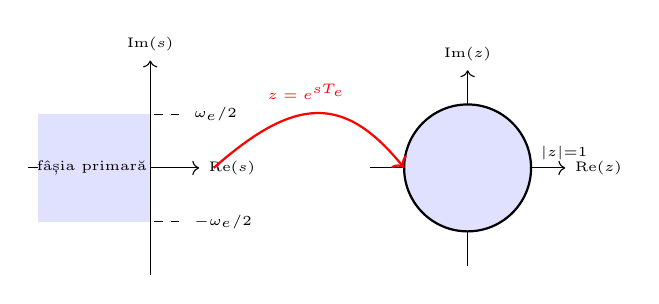
\begin{tikzpicture}[scale=0.62]
\draw[->] (-2.5,0) -- (1,0) node[right]{\tiny Re$(s)$};
\draw[->] (0,-2.2) -- (0,2.2) node[above]{\tiny Im$(s)$};
\draw[dashed] (-2.3,1.1)--(0.7,1.1); \node[right] at (0.7,1.1){\tiny $\omega_e/2$};
\draw[dashed] (-2.3,-1.1)--(0.7,-1.1); \node[right] at (0.7,-1.1){\tiny $-\omega_e/2$};
\fill[blue!12] (-2.3,-1.1) rectangle (0,1.1);
\node at (-1.2,0){\tiny fâșia primară};
\begin{scope}[xshift=6.5cm]
\draw[->] (-2,0) -- (2,0) node[right]{\tiny Re$(z)$};
\draw[->] (0,-2) -- (0,2) node[above]{\tiny Im$(z)$};
\fill[blue!12] (0,0) circle (1.3);
\draw[thick] (0,0) circle (1.3);
\node[right] at (1.3,0.3){\tiny $|z|{=}1$};
\end{scope}
\draw[->,thick,red] (1.3,0) .. controls (3,1.5) and (4,1.5) .. (5.2,0);
\node[above,red] at (3.2,1.2){\tiny $z=e^{sT_e}$};
\end{tikzpicture}
\end{center}

\section*{10. Scheme bloc echivalente pentru sisteme discrete}\phantomsection\label{sec:10}
\srcnote{curs 6, secțiunea 4.6.4.1 + seminar 3, exercițiul 6 (fig. 4.39 — derivare completă pentru reacție neunitară cu regulator numeric).}
\textbf{Serie, cu eșantionor intercalat} (Fig. 4.37a): $G_{es}(z)=G_1(z)G_2(z)$.\\
\textbf{Serie, fără eșantionor intercalat} (Fig. 4.37b): $G_{es}(z)=\overline{G_1G_2}(z)=Z\{G_1(s)G_2(s)\}$.
\begin{keyeq}\color{red!65!black}
$$G_1(z)G_2(z)\;\ne\;\overline{G_1G_2}(z)\qquad\text{(atenție: ordinea/prezența eșantionoarelor contează!)}$$
\end{keyeq}
\textbf{Reacție negativă neunitară, cu eșantionarea erorii:}
\begin{keyeq}\color{red!65!black}
$$G_{er}(z)=\dfrac{Y(z)}{R(z)}=\dfrac{G(z)}{1+GH(z)}\qquad\text{unde } GH(z)=Z\{G(s)H(s)\}$$
\end{keyeq}
Proprietăți operator eșantionare: $[U_1(s){\pm}U_2(s)]^*=U_1^*(s){\pm}U_2^*(s)$; $(U^*(s))^*=U^*(s)$; $[G(s)U^*(s)]^*=G^*(s)U^*(s)$.

\section*{11. Stabilitatea sistemelor discrete}\phantomsection\label{sec:11}
\srcnote{nu apare într-un curs numerotat din setul disponibil (cursurile 1–7 și 12; probabil curs 8/9, indisponibil aici) — conținut standard (criteriul cercului unitar, transformarea $r$ + Routh-Hurwitz), verificat pe o problemă rezolvată din notițele de recapitulare (seminar 7, tablou Routh complet în $r$).}
\textbf{Criteriul cercului unitar:} sistemul discret în circuit închis e stabil $\iff$ toți polii lui $G_{er}(z)$ (rădăcinile ecuației caracteristice $1+GH(z)=0$) sunt \textbf{în interiorul} cercului de rază unitară ($|z_i|<1$). Pe cerc $\to$ limită de stabilitate; în afară $\to$ instabil.

\textbf{Transformarea biliniară $r$ (sau $w$) + Routh-Hurwitz:} pentru a aplica R-H (definit pentru semiplanul stâng), se face schimbarea de variabilă
\begin{keyeq}\color{red!65!black}
$$z=\dfrac{r+1}{r-1}\quad\Big(\text{echivalent } r=\dfrac{z+1}{z-1}\Big)\qquad\text{(interior cerc unitar }|z|{<}1\;\longleftrightarrow\; \mathrm{Re}(r)<0\text{, SCS)}$$
\end{keyeq}
apoi se scrie ecuația caracteristică $A(z)\to A_r(r)$ și se aplică tabloul Routh clasic în $r$: sistem stabil $\iff$ toți termenii primei coloane au același semn; nr. schimbări de semn = nr. rădăcini în afara cercului. Dacă un rând se anulează complet, se înlocuiește cu derivata polinomului auxiliar (rândul anterior), la fel ca la R-H continuu.

\textbf{Exemplu} (Seminar 4): $A_z(z)=(z-1)(z-0{,}5)(z-2)=z^3-3{,}5z^2+3{,}5z-1$ — direct din factorizare: rădăcina $z=1$ e \emph{pe} cerc și $z=2$ e \emph{în afara} cercului unitar $\Rightarrow$ deja se vede că sistemul e instabil. Verificare cu Routh: cu $z=(r+1)/(r-1)$ se obține $A_r(r)=(r-1)^3A_z\big(\tfrac{r+1}{r-1}\big)=9-r^2$ (grad 2, nu 3 — rădăcina $z{=}1$ „dispare" la $r=\infty$). Tablou Routh pentru $r^2-9$ (semn schimbat, nu contează pentru stabilitate):
$$\begin{array}{c|cc} r^2 & 1 & -9\\ r^1 & 0\to2 & 0\\ r^0 & -9 & \end{array}$$
(rândul $r^1$ nul $\Rightarrow$ înlocuit cu derivata $\tfrac{d}{dr}(r^2-9)=2r$, coeficient $2$) — prima coloană $1,\,2,\,-9$ are \textbf{o schimbare de semn} (de la $+$ la $-$) $\Rightarrow$ o rădăcină în semiplanul drept $\Rightarrow$ \textbf{sistem instabil} (rădăcinile exacte $r=\pm3$ corespund la $z=(r{+}1)/(r{-}1)\in\{2,\,0{,}5\}$, plus $z=1$ „ascunsă" la $r\to\infty$).

\section*{12. Eroarea staționară}\phantomsection\label{sec:12}
\srcnote{nu apare într-un curs numerotat din setul disponibil — conținut sintetizat din notițele de recapitulare (curs 13, aplicație rezolvată cu teorema valorii finale) și prin analogie cu eroarea staționară de la sistemele continue.}
Pentru reacție negativă unitară, eroarea în $z$: $E(z)=\dfrac{R(z)}{1+G(z)}$. Cu \textbf{teorema valorii finale} (necesită polii lui $(1-z^{-1})E(z)$ în interiorul cercului unitar):
\begin{keyeq}\color{red!65!black}
$$e_{ss}=\lim_{k\to\infty}e[k]=\lim_{z\to1}(1-z^{-1})E(z)=\lim_{z\to1}\dfrac{(z-1)R(z)}{z\big[1+G(z)\big]}$$
\end{keyeq}
\textbf{Coeficienți de eroare} (analog continuu, tipul sistemului = nr. de poli ai lui $G(z)$ în $z{=}1$):
\begin{itemize}
\item treaptă: $R(z)=\frac{z}{z-1}\Rightarrow e_{ss}=\dfrac{1}{1+K_p}$, $K_p=\lim_{z\to1}G(z)$ — finit dacă tip 0, altfel $e_{ss}=0$;
\item rampă: $R(z)=\frac{T_ez}{(z-1)^2}\Rightarrow e_{ss}=\dfrac{1}{K_v}$, $K_v=\lim_{z\to1}\dfrac{(z-1)}{T_e}G(z)$ — finit dacă tip 1;
\item parabolă: $e_{ss}=1/K_a$, $K_a=\lim_{z\to1}\dfrac{(z-1)^2}{T_e^2}G(z)$ — finit dacă tip 2.
\end{itemize}
\textit{Practic la examen:} se scrie direct $E(z)=R(z)/(1+G(z))$ cu $R(z)$ din tabelul de la secțiunea 5 și se aplică teorema valorii finale — nu trebuie memorate formulele $K_p,K_v,K_a$, rezultă automat.

\section*{13. Curba polară / caracteristicile amplitudine-pulsație și fază-pulsație}\phantomsection\label{sec:13}
\srcnote{nu apare într-un curs numerotat din setul disponibil — conținut sintetizat din bilete (secțiunile \hyperref[sec:17]{17}–\hyperref[sec:18]{18}) și prin analogie cu caracteristicile de frecvență de la sistemele continue.}
Se înlocuiește $z=e^{j\omega T_e}$ în $G_d(z)$ și se variază $\omega\in[0,\,\pi/T_e]$ (până la pulsația Nyquist — dincolo caracteristica se repetă/oglindește, fiind periodică).

\textit{Atenție la formularea exactă din enunț — apare în 2 variante echivalente ca și calcul, diferite ca reprezentare grafică finală:}
\begin{itemize}
\item \textbf{"curba polară"}: se trasează $\mathrm{Im}\{G_d(j\omega)\}$ funcție de $\mathrm{Re}\{G_d(j\omega)\}$, într-un singur plan complex (secțiunea de mai jos);
\item \textbf{"caracteristicile amplitudine-pulsație și fază-pulsație"}: se trasează \textbf{separat} $|G_d(j\omega)|$ funcție de $\omega$ și $\angle G_d(j\omega)$ funcție de $\omega$ (două grafice, ca la Bode dar nu neapărat în dB/scară log — modulul și faza sunt aceleași mărimi calculate la pasul (2) de mai jos, doar reprezentarea diferă).
\end{itemize}
\begin{keyeq}\color{red!65!black}
$$G_d(j\omega)=G_d(z)\big|_{z=e^{j\omega T_e}}=\mathrm{Re}\{G_d(j\omega)\}+j\,\mathrm{Im}\{G_d(j\omega)\}$$
\textbf{Punct de plecare} ($\omega{=}0,\ z{=}1$): $G_d(1)$ — real. \quad\textbf{Punct de sosire} ($\omega{=}\pi/T_e,\ z{=}-1$): $G_d(-1)$ — real.
\end{keyeq}
\textbf{Pași:} (1) se scrie $z=\cos\omega T_e+j\sin\omega T_e$ și se înlocuiește în $G_d(z)$; (2) se raționalizează (se amplifică cu conjugata numitorului) pentru a separa Re/Im; (3) se evaluează limitele la $\omega=0$ și $\omega=\pi/T_e$ (capetele curbei) și eventual intersecția cu axele; (4) se trasează curba în planul complex între aceste două puncte.

\textbf{Exemplu generic} — pentru $G_d(z)=\dfrac{a_1z+a_0}{z^2+b_1z+b_0}$: la $\omega{=}0$ ($z{=}1$): $G_d(1)=\dfrac{a_1+a_0}{1+b_1+b_0}$; la $\omega{=}\pi/T_e$ ($z{=}{-}1$): $G_d(-1)=\dfrac{-a_1+a_0}{1-b_1+b_0}$. Pentru Re/Im general se înmulțește cu conjugata numitorului $\big[(\cos\omega T_e{-}\cos^2{-}\sin^2{+}b_0)-jb_1\sin\omega T_e\big]$ ... etc. (se face numeric pas cu pas ca la exemplul din bilete, nu se memorează formă generală).

\section*{14. Locul rădăcinilor pentru sisteme discrete}\phantomsection\label{sec:14}
\srcnote{curs 12, secțiunea 4.10.}
Ecuația caracteristică $1+GH(z)=0$, adică $GH(z)=|GH(z)|e^{j\theta}=-1=1\cdot e^{j(2k+1)180^\circ}$, dă:
\begin{keyeq}\color{red!65!black}
\textbf{condiția modulului:} $|GH(z)|=1$ \qquad \textbf{condiția argumentului:} $\angle GH(z)=180^\circ(2k+1),\ k=0,1,\dots$
\end{keyeq}
Locul rădăcinilor = locul geometric al polilor sistemului închis când $K$ variază $0\to\infty$ în
$$GH(z)=K\dfrac{(z-z_1)\cdots(z-z_m)}{(z-p_1)\cdots(z-p_n)}$$

\textbf{Cei 8 pași (identici ca principiu cu sistemele continue):}
\begin{enumerate}
\item ecuația caracteristică $1+K\,B(z)/A(z)=0$, se izolează $K$;
\item nr. ramuri $=n$ (nr. poli GH); se plasează polii ($\times$) și zerourile ($\circ$); locul \emph{începe} în poli, \emph{se termină} în zerouri (finite sau la $\infty$);
\item pe axa reală: aparține locului porțiunea la \textbf{stânga unui număr impar} de poli+zerouri reale;
\item \textbf{asimptote}: nr. $=n-m$; unghiuri $\theta_k=\dfrac{180^\circ(2k+1)}{n-m}$; abscisa centrului $\sigma_a=\dfrac{\sum p_i-\sum z_j}{n-m}$;
\item \textbf{puncte de ramificație}: rădăcinile reale (de pe porțiunea din pasul 3) ale $\dfrac{dK}{dz}=0$, cu $K=-A(z)/B(z)$;
\item \textbf{unghi de plecare/sosire} dintr-un pol/zero complex: $\theta_p=180^\circ+\sum\varphi_j-\sum\theta_i$ (plecare), $\theta_s=180^\circ+\sum\theta_i-\sum\varphi_j$ (sosire) — $\varphi$ unghiuri din zerouri, $\theta$ unghiuri din poli;
\item \textbf{intersecția cu cercul unitar}: cu Routh-Hurwitz modificat (transformarea $r$, secțiunea 11) sau rezolvând $1+K\,B(e^{j\omega T_e})/A(e^{j\omega T_e})=0$ pentru $\omega,K$;
\item \textbf{gradare}: $K=1/|GH(z_1)|=|A(z_1)/B(z_1)|$ în orice punct $z_1$ de pe loc.
\end{enumerate}

\textbf{Proprietate generală, 2 poli reali + 1 zero real (des cerută la Sub.\,3 din bilete — vezi secțiunea \hyperref[sec:16]{16}):} pentru $GH(z)=K\dfrac{z-z_0}{(z-p_1)(z-p_2)}$ (reacție unitară, $p_1,p_2,z_0\in\mathbb R$), \textbf{porțiunea complexă a locului rădăcinilor este întotdeauna un cerc centrat chiar în zero $z_0$}, de rază
\begin{keyeq}\color{red!65!black}
$$(x-z_0)^2+y^2=R^2,\qquad R=\sqrt{(z_0-p_1)(z_0-p_2)}\qquad(z=x+jy)$$
\end{keyeq}
\textbf{Demonstrație:} din ecuația caracteristică $ (z-p_1)(z-p_2)+K(z-z_0)=0$, cu $z=x+jy$: partea imaginară dă $y\big[2x-(p_1{+}p_2)+K\big]=0$, deci (pt. $y\ne0$) $K=(p_1{+}p_2)-2x$; înlocuind în partea reală și grupând termenii pătratici se obține direct $(x-z_0)^2+y^2=(z_0-p_1)(z_0-p_2)$, independent de $K$. Cazul particular $z_0{=}0$ (zero în origine, ex. $GH(z)=\frac{K(1{-}e^{-aT_e})z}{(z-1)(z-e^{-aT_e})}$, secțiunea \hyperref[sec:16]{16}) redă formula veche $x^2{+}y^2{=}e^{-aT_e}$; formula de mai sus e însă \textbf{valabilă pentru orice $z_0$} — vezi aplicațiile numerice din secțiunea \hyperref[sec:18]{18}.

\begin{center}
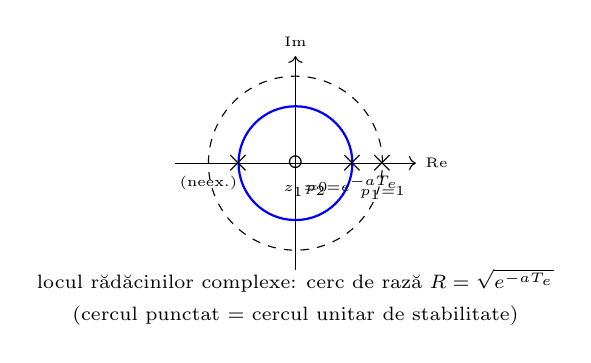
\begin{tikzpicture}[scale=0.85]
\draw[->] (-1.8,0) -- (1.8,0) node[right]{\tiny Re};
\draw[->] (0,-1.6) -- (0,1.6) node[above]{\tiny Im};
\draw[dashed] (0,0) circle (1.3);
\draw[thick,blue] (0,0) circle (0.85);
\node at (0.85,0){\large$\times$}; \node[below] at (0.85,-0.05){\tiny $p_2{=}e^{-aT_e}$};
\node at (-0.85,0){\large$\times$}; \node[below] at (-1.3,-0.05){\tiny(neex.)};
\node at (1.3,0){\large$\times$}; \node[below] at (1.3,-0.2){\tiny $p_1{=}1$};
\node at (0,0){\large$\circ$}; \node[below] at (0.15,-0.15){\tiny $z_1{=}0$};
\node[align=center] at (0,-2){\scriptsize locul rădăcinilor complexe: cerc de rază $R=\sqrt{e^{-aT_e}}$\\\scriptsize (cercul punctat = cercul unitar de stabilitate)};
\end{tikzpicture}
\end{center}

\section*{15. Model cu variabile de stare. Controlabilitate și observabilitate}\phantomsection\label{sec:15}
\srcnote{nu apare într-un curs numerotat din setul disponibil (probabil capitol separat, indisponibil aici) — forma companion e conținut standard de teoria sistemelor, verificat numeric pe exemplele din bilete (secțiunile \hyperref[sec:17]{17}–\hyperref[sec:18]{18}).}
Pentru $G(z)=\dfrac{b_{n-1}z^{n-1}+\dots+b_1z+b_0}{z^n+a_{n-1}z^{n-1}+\dots+a_1z+a_0}$ (strict propriu), \textbf{forma complet controlabilă (variabile de fază)}:
\begin{keyeq}\color{red!65!black}
$$x[k+1]=Ax[k]+Bu[k],\qquad y[k]=Cx[k]$$
$$A=\begin{pmatrix}0&1&0&\cdots&0\\0&0&1&\cdots&0\\\vdots&&&\ddots&\vdots\\-a_0&-a_1&-a_2&\cdots&-a_{n-1}\end{pmatrix},\ B=\begin{pmatrix}0\\\vdots\\0\\1\end{pmatrix},\ C=\begin{pmatrix}b_0&b_1&\cdots&b_{n-1}\end{pmatrix}$$
\end{keyeq}
Dacă $\deg(\text{numărător})=\deg(\text{numitor})=n$ (biproper, $G(z)=b_n+\dots$): se face împărțirea $B(z)=b_nA(z)+B'(z)$, se obține $D=b_n$ (transmisie directă) și se folosesc coeficienții reduși $b_i'=b_i-b_na_i$ în $C$.

\textbf{Controlabilitate:} $P=[\,B\;\;AB\;\;A^2B\;\cdots\;A^{n-1}B\,]$, sistem controlabil $\iff \mathrm{rang}\,P=n\iff\det P\ne0$.
\begin{keyeq}\color{red!65!black}
\textbf{Demonstrație generală:} pentru forma canonică controlabilă de mai sus, $P$ este \emph{întotdeauna} o matrice triunghiulară cu $\pm1$ pe anti-diagonală (indiferent de valorile $a_i$), deci $\det P=\pm1\ne0$ pentru orice sistem $\Rightarrow$ \textbf{forma cu variabile de fază este întotdeauna controlabilă}, prin construcție.
\end{keyeq}

\textbf{Observabilitate:} $Q=\begin{pmatrix}C\\CA\\\vdots\\CA^{n-1}\end{pmatrix}$, sistem observabil $\iff \mathrm{rang}\,Q=n\iff\det Q\ne0$ (spre deosebire de controlabilitate, observabilitatea \textbf{depinde efectiv} de valorile coeficienților — trebuie calculată de fiecare dată).

\textbf{Forma complet observabilă} (cerută direct în unele bilete, ex. secțiunea \hyperref[sec:18]{18} — nu doar verificarea cu $Q$ a formei controlabile de mai sus): se obține direct din matricele $(A,B,C)$ ale formei controlabile prin transpunere/schimbare de rol $B\leftrightarrow C$ (are aceeași funcție de transfer, $G(z)=G^T(z)$ fiind scalar la SISO):
\begin{keyeq}\color{red!65!black}
$$A_o=A^{T}=\begin{pmatrix}0&0&\cdots&0&-a_0\\1&0&\cdots&0&-a_1\\0&1&\cdots&0&-a_2\\\vdots&&\ddots&&\vdots\\0&0&\cdots&1&-a_{n-1}\end{pmatrix},\quad B_o=C^{T}=\begin{pmatrix}b_0\\b_1\\\vdots\\b_{n-1}\end{pmatrix},\quad C_o=B^{T}=\begin{pmatrix}0&\cdots&0&1\end{pmatrix}$$
\end{keyeq}
Prin construcție $Q_o=[C_o^T\ A_o^TC_o^T\ \cdots]^T$ e triunghiulară cu $\pm1$ pe anti-diagonală (analog cu $P$ la forma controlabilă) $\Rightarrow$ \textbf{forma complet observabilă e întotdeauna observabilă}; \emph{controlabilitatea} ei depinde efectiv de coeficienți (rolurile se inversează față de forma controlabilă) — se verifică analog cu $P_o=[B_o\ A_oB_o\ \cdots]$.

\textbf{Exemplu numeric (subiect tip din bilete):} $G_0(z)=\dfrac{0{,}02z+0{,}01}{z^2-1{,}51z+0{,}54}$ ($a_1{=}{-}1{,}51,\,a_0{=}0{,}54,\,b_1{=}0{,}02,\,b_0{=}0{,}01$):
$$A=\begin{pmatrix}0&1\\-0{,}54&1{,}51\end{pmatrix},\ B=\begin{pmatrix}0\\1\end{pmatrix},\ C=\begin{pmatrix}0{,}01&0{,}02\end{pmatrix}$$
$P=[B\ AB]=\begin{pmatrix}0&1\\1&1{,}51\end{pmatrix}$, $\det P=-1\ne0\Rightarrow$ \textbf{controlabil}. $CA=(0{,}01{\cdot}0{+}0{,}02{\cdot}({-}0{,}54)\ \ 0{,}01{\cdot}1{+}0{,}02{\cdot}1{,}51)=({-}0{,}0108\ \ 0{,}0402)$, $Q=\begin{pmatrix}0{,}01&0{,}02\\-0{,}0108&0{,}0402\end{pmatrix}$, $\det Q=0{,}000618\ne0\Rightarrow$ \textbf{observabil}.

\textbf{Caz biproper} (alt bilet): $G_0(z)=\dfrac{z^2-1{,}39z+0{,}52}{z^2-1{,}43z+0{,}49}$ ($a_1{=}{-}1{,}43,a_0{=}0{,}49,b_2{=}1,b_1{=}{-}1{,}39,b_0{=}0{,}52$): $D=b_2=1$; $b_1'=b_1-b_2a_1=-1{,}39+1{,}43=0{,}04$; $b_0'=b_0-b_2a_0=0{,}52-0{,}49=0{,}03$ $\Rightarrow$
$$A=\begin{pmatrix}0&1\\-0{,}49&1{,}43\end{pmatrix},\ B=\begin{pmatrix}0\\1\end{pmatrix},\ C=\begin{pmatrix}0{,}03&0{,}04\end{pmatrix},\ D=1$$
\textit{Schema bloc din model:} 2 integratoare (blocuri $z^{-1}$) în cascadă pentru $x_1,x_2$, cu reacții $-a_0,-a_1$ pe intrare și sumator de ieșire cu câștigurile $b_0',b_1'$ (plus ramura directă $D$ dacă există).

\section*{16. Fișă rapidă — subiectele recurente în bilete (toamnă 2022 – vară 2026, 6 bilete analizate)}\phantomsection\label{sec:16}
Din cele 6 bilete disponibile (toamnă 2022, vară 2024, și 4 bilete din sesiunea vară 2026 — vezi secțiunile \hyperref[sec:17]{17} și \hyperref[sec:18]{18}): structura e \textbf{fixă pe 4 subiecte + 5 întrebări de teorie (1p fiecare)}, doar valorile numerice, \emph{metoda cerută la Sub.\,1} și \emph{formularea Sub.\,2} diferă între bilete.

\begin{keyeq}\color{red!65!black}
\textbf{Sub. 1 — sistem cu $E^*(s),G(s)$, ERO:} (a) funcția de transfer în circuit închis prin \textbf{una din metodele secțiunii 8} (matched \textbf{sau} metoda trapezului \textbf{sau} metoda integrării — citește enunțul!); (b) tipul de intrare cu eroare staționară finită (secțiunea 12, teorema valorii finale pe $E(z)=1/(1+G_d(z))\cdot R(z)$, unde $G_d(z)$ e cea găsită la (a)); (c) răspunsul la treaptă (sau impuls) unitară — transformata Z inversă (secțiunea 6) aplicată lui $Y(z)=G_{er}(z)R(z)$.
\end{keyeq}

\begin{keyeq}\color{red!65!black}
\textbf{Sub. 2 — pentru $G_d(z)$ dat (reacție unitară), citește exact ce cere enunțul:} \textbf{fie} "curba polară" (parte reală/imaginară — secțiunea 13 pas 1-2; punct plecare $G_d(1)$ / sosire $G_d(-1)$; trasare curbă), \textbf{fie} "caracteristicile amplitudine-pulsație și fază-pulsație" (aceleași Re/Im calculate, dar trasate ca $|G_d(j\omega)|$ și $\angle G_d(j\omega)$ separat, funcție de $\omega$) — vezi secțiunea 13.
\end{keyeq}

\begin{keyeq}\color{red!65!black}
\textbf{Sub. 3 — locul rădăcinilor pentru $G_d(z)=k\,B(z)/A(z)$ (reacție unitară), din enunț cu $k$ parametru:} toți cei 8 pași din secțiunea 14 — (a) nr. ramuri + poli/zerouri; (b) porțiune axă reală; (c) nr. asimptote + unghi + centroid; (d) puncte ramificație; (e) verificare cerc + trasare (verifică mereu proprietatea specială din secțiunea 14 dacă zeroul e în $z{=}0$ și sunt 2 poli reali!).
\end{keyeq}

\begin{keyeq}\color{red!65!black}
\textbf{Sub. 4 — $G_0(z)$ în circuit închis dat direct:} (a) model cu variabile de stare, forma complet controlabilă + \textbf{demonstrația} generală (secțiunea 15 — $\det P=\pm1$ mereu); (b) \textbf{fie} verificare observabilitate cu matricea $Q$ (calcul explicit, secțiunea 15), \textbf{fie} schema bloc a realizării (integratoare + sumatoare din $A,B,C$) — ambele variante au apărut, verifică cerința exactă din enunț.
\end{keyeq}

\begin{keyeq}\color{red!65!black}
\textbf{Teorie (1p fiecare, identice/foarte similare la toate biletele):}
\begin{enumerate}
\item transformarea planului $s$ în planul $z$ (secțiunea 9) — SCS $\to$ interiorul cercului unitar;
\item schema bloc funcțională a unui sistem de reglare numeric (secțiunea 1);
\item frecvența minimă de eșantionare / condiția de a nu avea aliasing = teorema Shannon (secțiunea 2);
\item rolul convertorului numeric-analogic = reface semnalul continuu, filtrează componentele de frecvență înaltă (secțiunea 4);
\item reprezentarea într-o schemă bloc a unui eșantionor ideal = comutator sincron cu perioadă $T_e$ (secțiunea 2);
\item (variantă) etapele conversiei analog-numerice = eșantionare + cuantizare + codificare (secțiunile 2-3);
\item (variantă) elementele specifice unui sistem numeric = CA/N, CN/A, ERO (secțiunea 1, 4);
\item (variantă) refacerea unui semnal continuu din eșantioanele sale folosind ERO = extrapolare cu ultima valoare (secțiunea 4).
\end{enumerate}
\end{keyeq}

\textit{Notă de ultim moment:} toate cele 6 bilete analizate au \textbf{aceeași structură pe 4 subiecte + teorie}; dacă mai găsești subiecte din 2025/2026, verifică întâi dacă tiparul s-a păstrat — dacă da, secțiunile 8 (familia de metode), 13, 14 și 15 de mai sus acoperă tot ce poate varia numeric.

\textbf{Observație numerică utilă (Sub.\,1, metoda trapezului, familia $G(s)=1/(s(s+b))$, $T_e{=}0{,}1$s):} indiferent de $b$, se obține mereu $G_d(z)=\dfrac{(z+1)^2}{(400+20b)z^2-800z+(400-20b)}$ — \textbf{coeficientul lui $z$ la numitor e mereu $-800$}, doar termenii extremi depind de $b$; util ca verificare rapidă de calcul la examen (vezi aplicația $b{=}5$ din secțiunea \hyperref[sec:17]{17} și $b{=}6$ din secțiunea \hyperref[sec:18]{18}).

\section*{17. Bilet oficial recent (sesiunea vară 2026) — foarte important!}\phantomsection\label{sec:17}
\textit{Bilet dat efectiv în acest an universitar; structura (4 subiecte + 5 întrebări de teorie, 1p fiecare) confirmă tiparul din secțiunea 16 și e cea mai probabilă pentru examenul curent. Teoria de la acest bilet e identică cu lista din secțiunea 16 (itemii 1,2,6,7,5) — nu se repetă mai jos.}

\begin{keyeq}\color{red!65!black}
\textbf{Subiect 1 — $G(s)=\dfrac1{s(s+5)}$, $T_e{=}0{,}1$s, schema cu eșantionarea erorii + ERO (secțiunea 1):}

\textbf{a) F.d.t. în circuit închis prin metoda trapezului} (secțiunea 8C: $s\to\dfrac2{T_e}\dfrac{z-1}{z+1}=20\dfrac{z-1}{z+1}$, aplicată direct pe $G(s)$):
$$\sigma=20\dfrac{z-1}{z+1}\ \Rightarrow\ \sigma(\sigma{+}5)=\dfrac{100(z-1)(5z-3)}{(z+1)^2}\ \Rightarrow\ G_d(z)=\dfrac{(z+1)^2}{500(z-1)(z-0{,}6)}=\dfrac{z^2+2z+1}{500z^2-800z+300}$$
Circuit închis (reacție unitară): $G_{er}(z)=\dfrac{G_d(z)}{1+G_d(z)}=\dfrac{(z+1)^2}{501z^2-798z+301}$ — poli $z_{1,2}\approx0{,}979;\ 0{,}613$ (în cercul unitar $\Rightarrow$ stabil).

\textbf{b) Eroare staționară finită:} $G_d(z)$ are un pol la $z{=}1$ (tip $\nu{=}1$, de la integratorul $1/s$). Cu $E(z){=}R(z)/(1{+}G_d(z))$ și teorema valorii finale (secțiunea 12): la \textbf{treaptă} $e_{ss}{=}0$; la \textbf{rampă} $e_{ss}{=}\lim_{z\to1}\dfrac{50(z-0{,}6)}{501z^2-798z+301}=\dfrac{50\cdot0{,}4}{4}=5$ (finită, nenulă!) $\Rightarrow$ \textbf{răspunsul căutat: intrare rampă} (la parabolă $e_{ss}{=}\infty$).

\textbf{c) Răspunsul la impuls Dirac unitar} ($R(z){=}1\Rightarrow Y(z){=}G_{er}(z)$): împărțind $\dfrac{z^2+2z+1}{501z^2-798z+301}=\dfrac1{501}+\dfrac{1800z+200}{501(501z^2-798z+301)}$ și descompunând partea proprie (secțiunea 6, metoda reziduurilor, $p_1{=}0{,}9793,p_2{=}0{,}6135$):
$$y[0]=\dfrac1{501}\approx0{,}002,\qquad y[k]=0{,}02138\,p_1^{\,k-1}-0{,}01421\,p_2^{\,k-1}\ \ (k\ge1)$$
Numeric: $y[1]{\approx}0{,}0072$, urcă lin până la un maxim ${\approx}0{,}018$ în jurul lui $k{\approx}7$-$8$, apoi scade \textbf{foarte lent} spre $0$ (constanta de timp $\sim1/(1{-}p_1){\approx}48$ eșantioane — polul $p_1{\approx}0{,}98$ e aproape de $1$, moștenire a integratorului din $G(s)$).
\end{keyeq}

\begin{center}
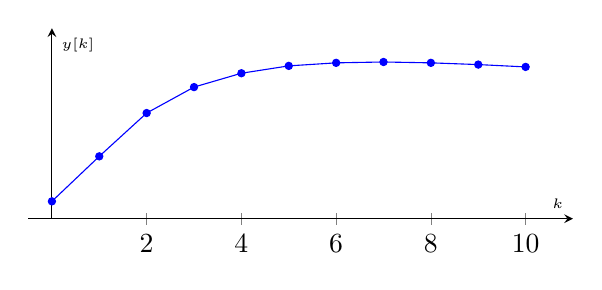
\begin{tikzpicture}
\begin{axis}[width=8.5cm,height=4cm,axis lines=middle,xlabel={\tiny $k$},ylabel={\tiny $y[k]$},xtick={0,2,4,6,8,10},ytick=\empty,ymin=0,ymax=0.022,xmin=-0.5,xmax=11,scatter/classes={a={mark=*,blue,mark size=1.3pt}}]
\addplot[scatter,only marks,scatter src=explicit symbolic] table[meta=lbl]{
x y lbl
0 0.002 a
1 0.0072 a
2 0.0122 a
3 0.0152 a
4 0.0168 a
5 0.01765 a
6 0.0180 a
7 0.0181 a
8 0.0180 a
9 0.0178 a
10 0.01753 a
};
\draw[blue] (axis cs:0,0.002)--(axis cs:1,0.0072)--(axis cs:2,0.0122)--(axis cs:3,0.0152)--(axis cs:4,0.0168)--(axis cs:5,0.01765)--(axis cs:6,0.018)--(axis cs:7,0.0181)--(axis cs:8,0.018)--(axis cs:9,0.0178)--(axis cs:10,0.01753);
\end{axis}
\end{tikzpicture}
\end{center}
\textit{Observație desen:} urcare rapidă din $y[0]{\approx}0$, platou larg $\approx0{,}018$, apoi coadă foarte lungă spre $0$ — tipic pentru sisteme cu pol închis aproape de cercul unitar.

\begin{keyeq}\color{red!65!black}
\textbf{Subiect 2 — caracteristici amplitudine-pulsație/fază-pulsație pentru $G_d(z)=\dfrac{0{,}2z+0{,}07}{z^2-0{,}5z+0{,}05}$, $T_e{=}1$s:}

Se înlocuiește $z{=}e^{j\omega}$ (secțiunea 13), $\omega\in[0,\pi]$ (Nyquist, $T_e{=}1\Rightarrow\omega_N{=}\pi$). Puncte cheie (calcul direct Re/Im, ca la exemplul din secțiunea 13):
\begin{center}\small
\begin{tabular}{c|ccccc}
$\omega$ & $0$ & $\pi/4$ & $\pi/2$ & $3\pi/4$ & $\pi$\\\hline
$|G_d(j\omega)|$ & $0{,}491$ & $0{,}356$ & $0{,}197$ & $0{,}112$ & $0{,}084$\\
$\angle G_d(j\omega)$ & $0^\circ$ & $-81{,}4^\circ$ & $-137{,}1^\circ$ & $-169{,}8^\circ$ & $180^\circ$\\
\end{tabular}
\end{center}
$G_d(1){=}0{,}27/0{,}55{=}0{,}491$ (punct plecare, real); $G_d(-1){=}{-}0{,}13/1{,}55{=}{-}0{,}084$ (punct sosire, real) — ambele confirmă modulul/faza din tabel la capete. Modulul scade monoton, faza scade monoton de la $0^\circ$ la $-180^\circ$.
\end{keyeq}

\begin{center}
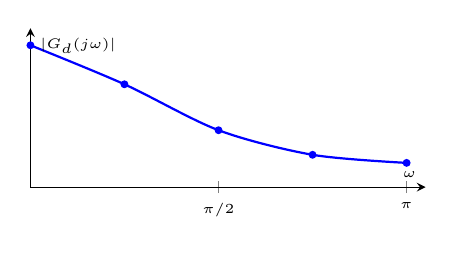
\begin{tikzpicture}
\begin{axis}[width=6.6cm,height=3.6cm,axis lines=middle,xlabel={\tiny $\omega$},ylabel={\tiny $|G_d(j\omega)|$},xtick={0,1.57,3.14},xticklabels={\tiny0,\tiny$\pi/2$,\tiny$\pi$},ytick=\empty,ymin=0,ymax=0.55,xmin=0,xmax=3.3]
\addplot[blue,thick,smooth,mark=*,mark size=1pt] coordinates {(0,0.491) (0.785,0.356) (1.571,0.197) (2.356,0.112) (3.1416,0.084)};
\end{axis}
\end{tikzpicture}
\hspace{2mm}
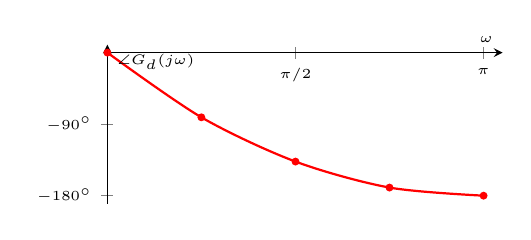
\begin{tikzpicture}
\begin{axis}[width=6.6cm,height=3.6cm,axis lines=middle,xlabel={\tiny $\omega$},ylabel={\tiny $\angle G_d(j\omega)$},xtick={0,1.57,3.14},xticklabels={\tiny0,\tiny$\pi/2$,\tiny$\pi$},ytick={0,-90,-180},yticklabels={\tiny0,\tiny$-90^\circ$,\tiny$-180^\circ$},ymin=-190,ymax=10,xmin=0,xmax=3.3]
\addplot[red,thick,smooth,mark=*,mark size=1pt] coordinates {(0,0) (0.785,-81.4) (1.571,-137.1) (2.356,-169.8) (3.1416,-180)};
\end{axis}
\end{tikzpicture}
\end{center}

\begin{keyeq}\color{red!65!black}
\textbf{Subiect 3 — locul rădăcinilor pentru $G_d(z)=\dfrac{k(0{,}13z+0{,}02)}{z^2-0{,}39z+0{,}007}$, $T_e{=}1$s (reacție unitară):}

Poli: $p_1{=}0{,}3711,\,p_2{=}0{,}0189$ (din $z^2{-}0{,}39z{+}0{,}007{=}0$). Zero: $z_0{=}{-}0{,}02/0{,}13{=}{-}0{,}1538$.

\textbf{a) Ramuri:} $n{=}2$ (câte poli), încep în $p_1,p_2$ ($k{=}0$); una se termină în $z_0$ ($k\to\infty$), cealaltă la $-\infty$ ($n{-}m{=}1$ ramură la infinit).

\textbf{b) Axa reală:} segmentele $[0{,}0189;\,0{,}3711]$ (între poli) și $(-\infty,\,-0{,}1538]$ (de la zero la $-\infty$).

\textbf{c) Asimptote:} $n{-}m{=}1$, unghi $180^\circ$ (axa reală negativă) — cu o singură asimptotă, ramura spre $\infty$ chiar \textbf{coincide} cu axa reală de la zero la $-\infty$ (nu există alt punct de întâlnire; centrul formal $\sigma_a{=}\frac{(p_1+p_2)-z_0}{1}{=}0{,}544$ e fără semnificație geometrică aici).

\textbf{d) Puncte de ramificație:} \textbf{breakaway} (între poli, ram. se ciocnesc) și \textbf{break-in} (înapoi pe axă, înainte de a se despărți spre $z_0$ și $-\infty$) — coordonatele exacte rezultă direct din cercul de la punctul (e): $x{=}z_0\pm R$.

\textbf{e) Verificare cerc — DA:} eliminând $k$ din ecuația caracteristică $z^2{-}0{,}39z{+}0{,}007{+}k(0{,}13z{+}0{,}02){=}0$ (condiția $k\in\mathbb R$, secțiunea metodei din text) rezultă exact:
$$(x+0{,}1538)^2+y^2=0{,}0907=R^2,\qquad R=\sqrt{(z_0{-}p_1)(z_0{-}p_2)}=0{,}301$$
— \textbf{cerc centrat chiar în zero} $z_0{=}{-}0{,}1538$! Intersecțiile cu axa reală (breakaway/break-in): $x{=}{-}0{,}1538\pm0{,}301\Rightarrow z{\approx}0{,}147$ ($k{\approx}0{,}73$) și $z{\approx}{-}0{,}455$ ($k{\approx}10{,}0$) — pentru $k\in(0{,}73;\,10{,}0)$ rădăcinile sunt complexe, pe cerc; în afara acestui interval, reale, pe segmentele de la (b).
\end{keyeq}

\begin{center}
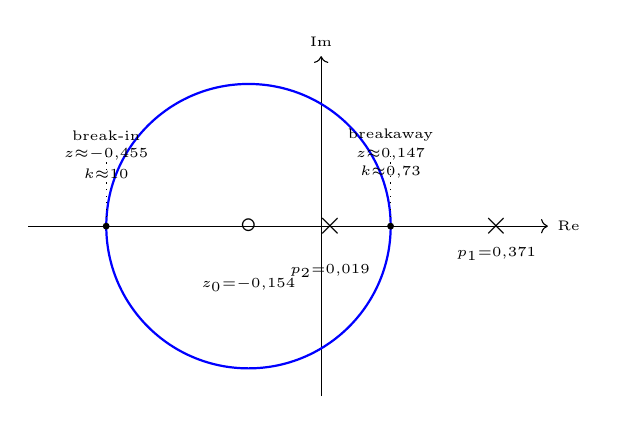
\begin{tikzpicture}[scale=6]
\draw[->] (-0.62,0) -- (0.48,0) node[right]{\tiny Re};
\draw[->] (0,-0.36) -- (0,0.36) node[above]{\tiny Im};
\draw[thick,blue] (-0.1538,0) circle (0.301);
\node at (0.3711,0){\large$\times$}; \node[below] at (0.3711,-0.025){\tiny $p_1{=}0{,}371$};
\node at (0.0189,0){\large$\times$}; \node[below] at (0.0189,-0.06){\tiny $p_2{=}0{,}019$};
\node at (-0.1538,0){\large$\circ$}; \node[below] at (-0.1538,-0.09){\tiny $z_0{=}{-}0{,}154$};
\filldraw (0.147,0) circle (0.006); \draw[dotted] (0.147,0.02)--(0.147,0.16);
\node[above] at (0.147,0.16){\tiny breakaway};
\node[above] at (0.147,0.12){\tiny $z{\approx}0{,}147$};
\node[above] at (0.147,0.08){\tiny $k{\approx}0{,}73$};
\filldraw (-0.455,0) circle (0.006); \draw[dotted] (-0.455,0.02)--(-0.455,0.16);
\node[above] at (-0.455,0.16){\tiny break-in};
\node[above] at (-0.455,0.12){\tiny $z{\approx}{-}0{,}455$};
\node[above] at (-0.455,0.08){\tiny $k{\approx}10$};
\end{tikzpicture}
\end{center}

\begin{keyeq}\color{red!65!black}
\textbf{Subiect 4 — $G_0(z)=\dfrac{0{,}02z+0{,}02}{z^2-1{,}49z+0{,}54}$ (circuit închis):} $a_1{=}{-}1{,}49,\,a_0{=}0{,}54,\,b_1{=}0{,}02,\,b_0{=}0{,}02$.

\textbf{a) Model SS, formă complet controlabilă} (secțiunea 15):
$$A=\begin{pmatrix}0&1\\-0{,}54&1{,}49\end{pmatrix},\ B=\begin{pmatrix}0\\1\end{pmatrix},\ C=\begin{pmatrix}0{,}02&0{,}02\end{pmatrix}$$
\textbf{Demonstrație controlabilitate:} $AB=\begin{pmatrix}1\\1{,}49\end{pmatrix}\Rightarrow P{=}[B\ AB]{=}\begin{pmatrix}0&1\\1&1{,}49\end{pmatrix}$, $\det P{=}{-}1\ne0$ — \textbf{întotdeauna} $\pm1$ pentru orice $a_0,a_1$ (formă companion, secțiunea 15) $\Rightarrow$ controlabil prin construcție.

\textbf{b) Observabilitate:} $CA=(0{,}02{\cdot}0{+}0{,}02{\cdot}({-}0{,}54)\ \ 0{,}02{\cdot}1{+}0{,}02{\cdot}1{,}49)=({-}0{,}0108\ \ 0{,}0298)$
$$Q=\begin{pmatrix}0{,}02&0{,}02\\-0{,}0108&0{,}0298\end{pmatrix},\qquad \det Q=0{,}02{\cdot}0{,}0298-0{,}02{\cdot}({-}0{,}0108)=0{,}000812\ne0\ \Rightarrow\ \textbf{observabil}$$
\end{keyeq}

\begin{center}
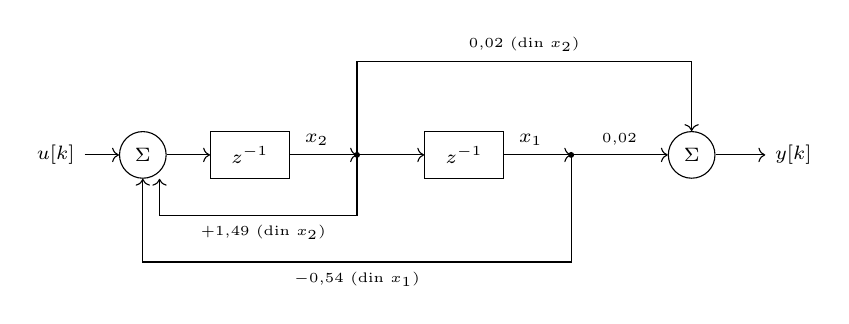
\begin{tikzpicture}[scale=0.85, every node/.style={font=\scriptsize}]
\node (u) at (0,0) {$u[k]$};
\node[draw,circle,minimum size=0.5cm] (s1) at (1.3,0) {$\Sigma$};
\draw[->] (u)--(s1);
\node[draw,minimum width=1cm,minimum height=0.6cm] (i1) at (2.9,0) {$z^{-1}$};
\draw[->] (s1)--(i1);
\coordinate (a) at (4.5,0);
\draw[->] (i1) -- (a) node[above,pos=0.4]{$x_2$};
\filldraw (a) circle (1pt);
\node[draw,minimum width=1cm,minimum height=0.6cm] (i2) at (6.1,0) {$z^{-1}$};
\draw[->] (a) -- (i2);
\coordinate (b) at (7.7,0);
\draw[->] (i2) -- (b) node[above,pos=0.4]{$x_1$};
\filldraw (b) circle (1pt);
\node[draw,circle,minimum size=0.5cm] (sy) at (9.5,0) {$\Sigma$};
\draw[->] (b) -- (sy) node[midway,above]{\tiny $0{,}02$};
\draw[->] (a) -- ++(0,1.4) -| (sy.north);
\node[above] at (7,1.4){\tiny $0{,}02$ (din $x_2$)};
\draw[->] (sy) -- (10.6,0) node[right]{$y[k]$};
\draw[->] (b) -- ++(0,-1.6) -| (s1.south);
\node[below] at (4.5,-1.6){\tiny $-0{,}54$ (din $x_1$)};
\draw[->] (a) -- ++(0,-0.9) -| ($(s1.south)+(0.25,0)$);
\node[below] at (3.1,-0.9){\tiny $+1{,}49$ (din $x_2$)};
\end{tikzpicture}
\end{center}

\section*{18. Alte 3 bilete (vară 2024 și vară 2026, bilete 1 \& 2 \& 4) — metoda matched complet rezolvată \& forma observabilă}\phantomsection\label{sec:18}
\textit{Aceste 3 bilete confirmă din nou tiparul pe 4 subiecte + teorie din secțiunea \hyperref[sec:16]{16}. Le tratăm concentrat: doar ce e \textbf{numeric nou} față de secțiunea \hyperref[sec:17]{17} (metoda matched aplicată efectiv, cu și fără integrator; forma SS observabilă cerută direct). Sub.\,2 și Sub.\,3 refolosesc exact formele din secțiunile \hyperref[sec:13]{13}/\hyperref[sec:14]{14}.}

\subsection*{18.1 Metoda matched, sistem \emph{fără} integrator (vară 2024): $G(s)=\dfrac1{s+4}$, $T_e{=}0{,}1$s}
Un singur pol finit $b{=}4$ (fără pol în $s{=}0$, deci $\nu{=}0$ — se folosește câștigul DC obișnuit, nu trucul cu $s^\nu$ din secțiunea \hyperref[sec:8]{8}). Nu sunt zerouri și $n{-}m{-}1{=}0$, deci \textbf{fără} factorul suplimentar $(z+1)$:
\begin{keyeq}\color{red!65!black}
$$z_d=e^{-4\cdot0,1}=0{,}67032,\qquad K_d=G(0)(1-z_d)=\tfrac14(1-0{,}67032)=0{,}08242\quad\Rightarrow\quad G_d(z)=\dfrac{0{,}08242}{z-0{,}67032}$$
\end{keyeq}
\textbf{b) tip de intrare cu eroare finită:} $G_d(z)$ nu are pol în $z{=}1$ (tip 0) $\Rightarrow$ la \textbf{treaptă}: $K_p{=}G_d(1){=}0{,}25$ (exact $G(0)$, cum trebuie prin construcția metodei matched), $e_{ss}=\dfrac1{1+K_p}=\dfrac1{1,25}=0{,}8$; la rampă $e_{ss}{=}\infty$.

\textbf{c) răspuns la treaptă unitară:} $G_{er}(z)=\dfrac{G_d(z)}{1+G_d(z)}=\dfrac{0{,}08242}{z-0{,}58790}$ (pol închis $0{,}5879{=}z_d{-}K_d$, stabil). Cu $Y(z)=G_{er}(z)\dfrac{z}{z-1}$, descompunere în fracții simple (secțiunea \hyperref[sec:6]{6}b) dă direct
\begin{keyeq}\color{red!65!black}
$$y[k]=0{,}2\big(1-0{,}5879^{\,k}\big),\ k\ge0\qquad\big(\text{coeficientul }0{,}2=\tfrac{G(0)}{1+G(0)}=1-e_{ss}\text{, verificare automată}\big)$$
\end{keyeq}

\begin{center}
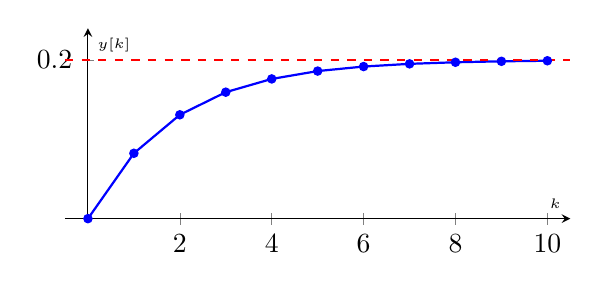
\begin{tikzpicture}
\begin{axis}[width=8cm,height=4cm,axis lines=middle,xlabel={\tiny $k$},ylabel={\tiny $y[k]$},xtick={0,2,4,6,8,10},ytick={0,0.2},ymin=0,ymax=0.24,xmin=-0.5,xmax=10.5]
\addplot[blue,thick,mark=*,mark size=1.3pt] coordinates {(0,0)(1,0.0824)(2,0.1309)(3,0.1594)(4,0.1761)(5,0.1860)(6,0.1917)(7,0.1951)(8,0.1971)(9,0.1983)(10,0.1990)};
\addplot[red,dashed] coordinates {(-0.5,0.2)(10.5,0.2)};
\end{axis}
\end{tikzpicture}
\end{center}
\textit{Observație desen:} urcare monoton crescătoare spre asimptota $y_\infty{=}0{,}2{=}1-e_{ss}$, tipic pt. sistem tip 0, pol unic $0{,}588$ (fără integrator, nu apare coada lungă de la sistemele cu pol lângă $1$).

\subsection*{18.2 Metoda matched, sistem \emph{cu} integrator (bilet 1, vară 2026): $G(s)=\dfrac1{s(s+9)}$, $T_e{=}0{,}1$s}
Pol finit $b{=}9\Rightarrow z_d=e^{-0,9}=0{,}40657$; polul din $s{=}0$ (integrator, $\nu{=}1$) dă mereu polul $z{=}1$; $n{-}m{-}1{=}1\Rightarrow$ se adaugă factorul $(z+1)$ la numărător:
\begin{keyeq}\color{red!65!black}
$$K_d:\ \ \lim_{s\to0}sG(s)=\tfrac19=\lim_{z\to1}\dfrac{z-1}{zT_e}G_d(z)\ \Rightarrow\ K_d=0{,}0032968\qquad G_d(z)=\dfrac{0{,}0032968(z+1)}{(z-1)(z-0{,}40657)}$$
\end{keyeq}
\textbf{b)} $G_d(z)$ are 1 pol în $z{=}1$ (tip 1) $\Rightarrow$ eroare finită la \textbf{rampă}: $e_{ss}=\lim_{z\to1}\dfrac{T_e}{(z-1)(1+G_d(z))}=9$ — exact $1/K_v$ cu $K_v{=}\lim_{s\to0}sG(s){=}1/9$ (verificare automată, la fel ca la subiectul din secțiunea \hyperref[sec:17]{17}).

\textbf{c) răspuns la impuls Dirac unitar} ($Y(z)=G_{er}(z)$):
$$G_{er}(z)=\dfrac{0{,}0032968(z+1)}{z^2-1{,}40327z+0{,}40987},\qquad p_1{=}0{,}98874,\ p_2{=}0{,}41454\ \ (\text{stabil})$$
Reziduuri (secțiunea \hyperref[sec:6]{6}a):
$$y[0]=0,\qquad y[k]=0{,}011419\,p_1^{\,k-1}-0{,}008122\,p_2^{\,k-1}\ \ (k\ge1)$$
\begin{center}\small
\begin{tabular}{c|cccccccc}
$k$ & 1 & 2 & 3 & 4 & 5 & 6 & 8 & 12\\\hline
$y[k]$ & $0{,}0033$ & $0{,}0079$ & $0{,}0098$ & $0{,}0105$ & $0{,}0107$ & $0{,}0107$ & $0{,}0105$ & $0{,}0102$
\end{tabular}
\end{center}
Urcare rapidă, platou $\approx0{,}0107$ în jurul lui $k{\approx}5$-$6$, apoi coadă \textbf{foarte lungă} spre $0$ ($p_1{\approx}0{,}989$, constantă de timp $\sim1/(1{-}p_1)\approx88$ eșantioane — moștenire a integratorului, exact fenomenul deja observat în secțiunea \hyperref[sec:17]{17}).

\textbf{d) forma SS complet controlabilă} pentru $G_{er}(z)$ de la (a)/(c) ($a_1{=}{-}1{,}40327,\,a_0{=}0{,}40987,\,b_1{=}b_0{=}0{,}0032968$):
$$A=\begin{pmatrix}0&1\\-0{,}40987&1{,}40327\end{pmatrix},\ B=\begin{pmatrix}0\\1\end{pmatrix},\ C=\begin{pmatrix}0{,}0032968&0{,}0032968\end{pmatrix}$$
$P{=}[B\ AB]{=}\begin{pmatrix}0&1\\1&1{,}40327\end{pmatrix}$, $\det P{=}{-}1\ne0\Rightarrow$ \textbf{controlabil} (mereu, cf. demonstrației generale din secțiunea \hyperref[sec:15]{15}).

\subsection*{18.3 Notă rapidă — Sub.\,1 la bilet 2 (vară 2026) și toamnă 2022}
Ambele folosesc \textbf{metoda trapezului} pe familia $G(s)=1/(s(s+b))$ din secțiunea \hyperref[sec:16]{16} (bilet 2: $b{=}3$; toamnă 2022: tot $b{=}3$), identic ca structură cu \hyperref[sec:17]{secțiunea 17} ($b{=}5$) și \hyperref[sec:18]{18.4} de mai jos ($b{=}6$) — doar se schimbă $b$ în formula generală. Pentru $b{=}3$: $G_d(z)=\dfrac{(z+1)^2}{460z^2-800z+340}$, poli deschis $1;\,0{,}7391$; poli închis (reacție unitară) $G_{er}(z)=\dfrac{(z+1)^2}{461z^2-798z+341}$, $p_{1,2}\approx0{,}9625;\,0{,}7685$ (ambii subunitari, stabil) — calculul complet e identic ca metodă cu \hyperref[sec:17]{secțiunea 17}, doar cu aceste valori numerice.

\subsection*{18.4 Metoda trapezului cu formă SS observabilă cerută (bilet 4, vară 2026): $G(s)=\dfrac1{s(s+6)}$, $T_e{=}0{,}1$s}
Din formula generală a secțiunii \hyperref[sec:16]{16} cu $b{=}6$: $G_d(z)=\dfrac{(z+1)^2}{520z^2-800z+280}$; circuit închis (reacție unitară):
\begin{keyeq}\color{red!65!black}
$$G_{er}(z)=\dfrac{(z+1)^2}{521z^2-798z+281},\qquad p_1{=}0{,}98299,\ p_2{=}0{,}54868\ \ (\text{stabil})$$
\end{keyeq}
Formă monică: $\dfrac{0{,}0019194z^2+0{,}0038388z+0{,}0019194}{z^2-1{,}53167z+0{,}53935}$ — \textbf{biproper} ($\deg$num$=\deg$den$=2$), deci $D{=}b_2{=}0{,}0019194$ și coeficienți reduși $b_1'=b_1-b_2a_1=0{,}0067786$, $b_0'=b_0-b_2a_0=0{,}0008842$ (secțiunea \hyperref[sec:15]{15}):
\begin{keyeq}\color{red!65!black}
\textbf{Forma complet controlabilă (intermediar):}\quad $A=\begin{pmatrix}0&1\\-0{,}53935&1{,}53167\end{pmatrix},\ B=\begin{pmatrix}0\\1\end{pmatrix},\ C=\begin{pmatrix}0{,}0008842&0{,}0067786\end{pmatrix},\ D=0{,}0019194$

\textbf{Forma complet observabilă cerută} ($A_o{=}A^T,\,B_o{=}C^T,\,C_o{=}B^T$, secțiunea \hyperref[sec:15]{15}):
$$A_o=\begin{pmatrix}0&-0{,}53935\\1&1{,}53167\end{pmatrix},\ B_o=\begin{pmatrix}0{,}0008842\\0{,}0067786\end{pmatrix},\ C_o=\begin{pmatrix}0&1\end{pmatrix},\ D_o=0{,}0019194$$
\end{keyeq}
\textbf{Demonstrație observabilitate (mereu adevărată):} $Q_o=[C_o^T\ \ A_o^TC_o^T]^T$ e triunghiulară cu $\pm1$ pe anti-diagonală (transpusa lui $P$ de la forma controlabilă, care era mereu $\det{=}\pm1$) $\Rightarrow\det Q_o=\pm1\ne0$, \textbf{observabilă prin construcție}, oricare ar fi $a_0,a_1$.

\textit{Schema bloc (formă observabilă, diferă topologic de forma controlabilă din secțiunea \hyperref[sec:17]{17}):} $x_2[k]$ e chiar ieșirea ($y{=}x_2{+}Du$); $x_2$ se obține integrând $x_1{-}a_1x_2{+}b_1'u$, iar $x_1$ se obține integrând $-a_0x_2{+}b_0'u$ — deci $u$ intră în \textbf{ambele} integratoare (prin $b_0',b_1'$), iar reacția $-a_0$ merge de la $x_2$ direct la intrarea primului integrator (nu mai e un simplu lanț cascadă ca la forma controlabilă).

\subsection*{18.5 Aplicații ale proprietății generale a cercului (secțiunea \hyperref[sec:14]{14}) — Sub.\,3 la bilet 1 și bilet 4}
\textbf{Bilet 1:} $G_d(z)=\dfrac{k(0{,}2z+0{,}07)}{z^2-0{,}5z+0{,}05}$ — poli $p_1{=}0{,}3618,\,p_2{=}0{,}1382$, zero $z_0{=}{-}0{,}35$. Cerc: $R=\sqrt{(z_0-p_1)(z_0-p_2)}=\sqrt{0{,}3475}=0{,}5895$, centrat în $z_0$. Breakaway/break-in: $x=z_0\pm R\Rightarrow 0{,}2395$ (între poli, $k{\approx}0{,}105$) și $-0{,}9395$ (pe ramura spre $-\infty$, $k{\approx}11{,}9$).

\textbf{Bilet 4:} $G_d(z)=\dfrac{0{,}368k(z+0{,}717)}{z^2-1{,}368z+0{,}368}$ — poli $p_1{=}1{,}0,\,p_2{=}0{,}368$, zero $z_0{=}{-}0{,}717$.
\begin{keyeq}\color{red!65!black}
$$R=\sqrt{(z_0-p_1)(z_0-p_2)}=\sqrt{1{,}8629}=1{,}3649\quad(\text{cerc mai mare decât cel unitar!})$$
\end{keyeq}
Breakaway (între poli) la $x{=}0{,}6479$ ($k{\approx}0{,}196$); break-in (pe ramura spre $-\infty$) la $x{=}{-}2{,}0819$ ($k{\approx}15{,}0$). Cum $R{>}1$, cercul locului rădăcinilor \textbf{iese din cercul unitar de stabilitate} — intersecția (rezolvând simultan cele două cercuri) e la $z{\approx}0{,}2433\pm j0{,}9700$, unde $k_{max}\approx2{,}40$: pentru $k\in(0{,}196;\,2{,}40)$ sistemul e stabil (rădăcini complexe în interiorul cercului unitar); peste $k{\approx}2{,}40$ sistemul devine \textbf{instabil} — o consecință directă utilă a proprietății generale, nu doar o curiozitate geometrică.

\begin{center}
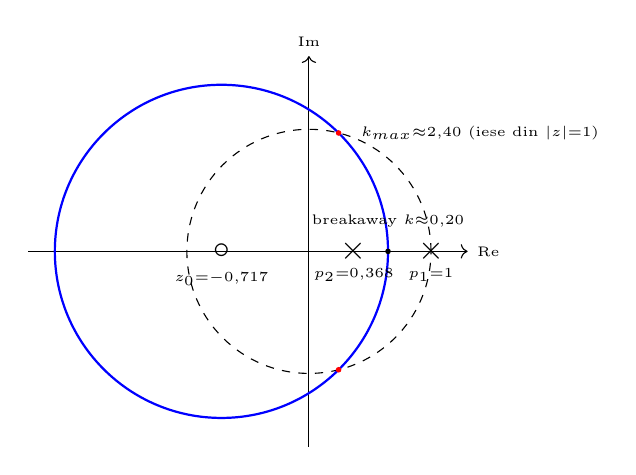
\begin{tikzpicture}[scale=1.55]
\draw[->] (-2.3,0) -- (1.3,0) node[right]{\tiny Re};
\draw[->] (0,-1.6) -- (0,1.6) node[above]{\tiny Im};
\draw[dashed] (0,0) circle (1);
\draw[thick,blue] (-0.717,0) circle (1.3649);
\node at (1.0,0){\large$\times$}; \node[below] at (1.0,-0.06){\tiny $p_1{=}1$};
\node at (0.368,0){\large$\times$}; \node[below] at (0.368,-0.06){\tiny $p_2{=}0{,}368$};
\node at (-0.717,0){\large$\circ$}; \node[below] at (-0.717,-0.09){\tiny $z_0{=}{-}0{,}717$};
\filldraw (0.648,0) circle (0.018); \node[above] at (0.648,0.12){\tiny breakaway $k{\approx}0{,}20$};
\filldraw[red] (0.243,0.970) circle (0.018); \filldraw[red] (0.243,-0.970) circle (0.018);
\node[right] at (0.35,0.97){\tiny $k_{max}{\approx}2{,}40$ (iese din $|z|{=}1$)};
\end{tikzpicture}
\end{center}

\end{document}
